\documentclass[a4paper,12pt,twoside]{memoir}
\usepackage{longtable}
\usepackage{btp}    % Use the trainermanual package option (i.e. \usepackage[trainermanual]{btp}) to generate the Trainer's version of the manual
%\usepackage[
%  noinfo,
%  cam,
%  cross,                % crosses as marks
%  a4,
%  width=6.25in,         % the width of the galley
%  height=9.25in,        % the height of the galley
%  center                % actual page is centered on the galley
%]{crop}
% Set some Workshop specific info
\setWorkshopTitle{A denovo Assembly Hands-on Workshop}
\setWorkshopVenue{}
\setWorkshopDate{}
\setWorkshopAuthor{
Bioplatforms Australia (BPA)\\
The Commonwealth Scientific and Industrial Research Organisation (CSIRO)\\
}

\begin{document}

%
% Workshop Title Page
%
\workshoptitlepage

%
% CC-BY
%
\input{licences/licence.tex}
\clearpage

\tableofcontents

\chapter{Workshop Information}
\clearpage

%
% Trainers Page
%
\section{The Trainers}

\newlength{\trainerIconWidth}
\setlength{\trainerIconWidth}{2.0cm}

\begin{center}
\begin{longtable}{>{\centering\arraybackslash} m{1.1\trainerIconWidth} m{1\textwidth}}


  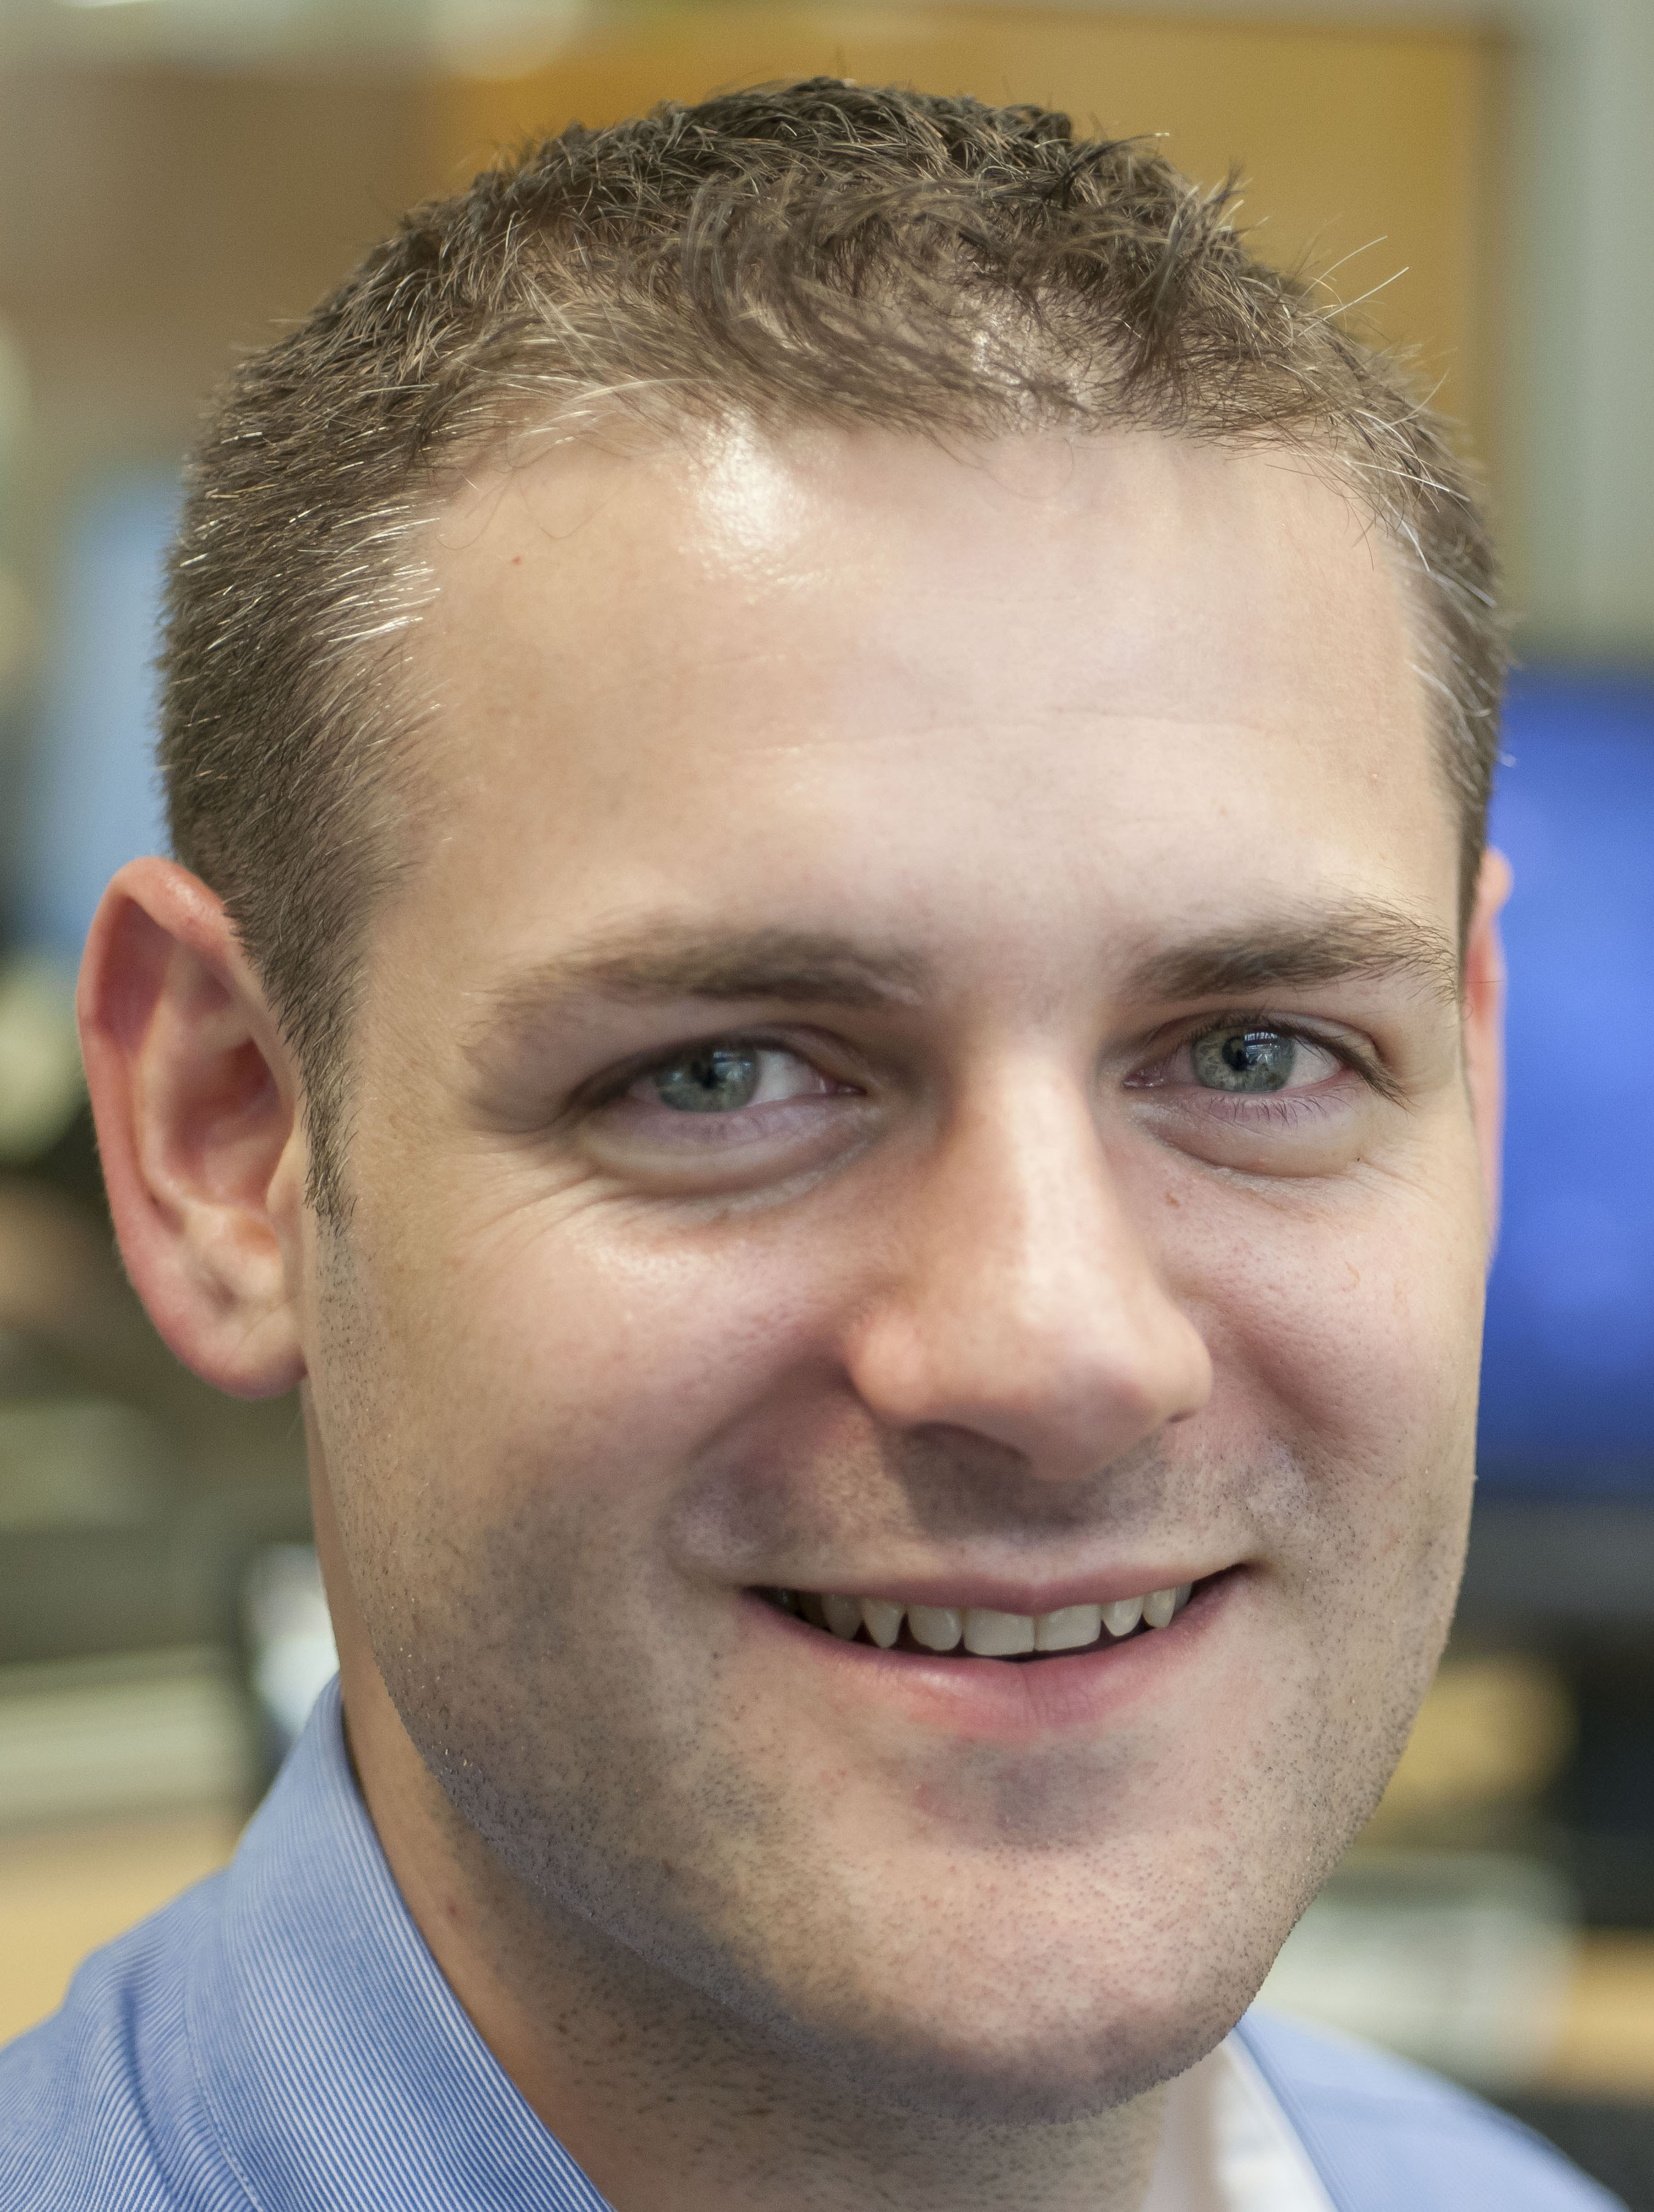
\includegraphics[width=\trainerIconWidth]{photos/Berkman.jpg} &
    \textbf{Dr. Paul Berkman}\newline
    Postion\newline
    CSIRO, The University of Queensland, Brisbane\newline
    \mailto{Paul.Berkman@csiro.au}\\

  \includegraphics[width=\trainerIconWidth]{photos/Chen.jpg} &
    \textbf{Dr. Zhiliang Chen}\newline
    Postdoctoral Research Associate\newline
    Systems Biology Initiative\newline
    The University of New South Wales (UNSW), NSW\newline
    \mailto{zhiliang@unsw.edu.au}\\

  
\includegraphics[width=\trainerIconWidth]{photos/Le.jpg} &
    \textbf{Mrs. Lien Le}\newline
    Senior Bioinformatics Manager\newline
    Bioinformatics Resource Australia EMBL and Research Computing Centre, UQ\newline
    \mailto{l.le2@uq.edu.au}\\

  \includegraphics[width=\trainerIconWidth]{photos/McGrath.jpg} &
    \textbf{Dr. Annette McGrath}\newline
    Bioinformatics Core Leader at CSIRO\newline
    Bioinformatics Core, CSIRO Mathematics, Informatics and Statistics, ACT\newline
    \mailto{Annette.Mcgrath@csiro.au}\\

  \includegraphics[width=\trainerIconWidth]{photos/McWilliam.jpg} & 
    \textbf{Mr. Sean McWilliam}\newline
    Bioinformatics Analyst\newline
    CSIRO Agriculture, QLD\newline
    \mailto{sean.mcwilliam@csiro.au}\\
    \pagebreak
  
  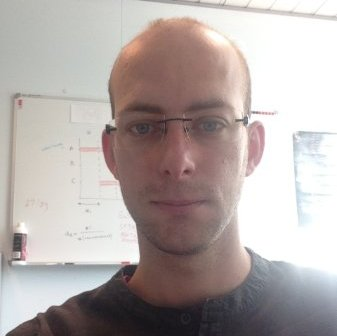
\includegraphics[width=\trainerIconWidth]{photos/Moncuet.jpg} &
    \textbf{Dr. Phillip Moncuet }\newline
    Position\newline
    The University of \newline
    \mailto{@.edu.au}\\

  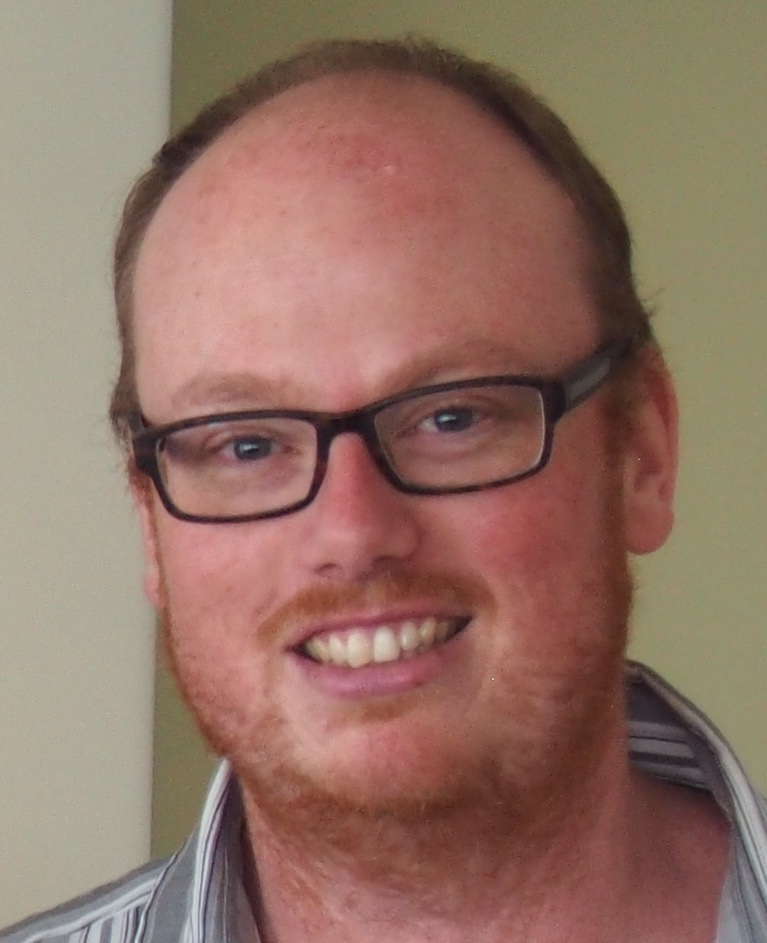
\includegraphics[width=\trainerIconWidth]{photos/Seeman.jpg} &
    \textbf{Dr.Torsten Seeman }\newline
    Associate Professor \newline
    The University \newline
    \mailto{@.edu.au}\\

  \includegraphics[width=\trainerIconWidth]{photos/Tyagi.jpg} & 
    \textbf{Dr. Sonika Tyagi}\newline
    Bioinformatics Supervisor\newline
    Australian Genome Research Facility Ltd, The Walter and Eliza Hall Institute, VIC\newline
    \mailto{sonika.tyagi@agrf.org.au}\\


\includegraphics[width=\trainerIconWidth]{photos/Revote.jpg} &
    \textbf{Mr. Jerico Revote }\newline
    e-Research Australia\newline
    Monash University, Clayton VIC\newline
    \mailto{jerico.revote@monash.edu}\\

  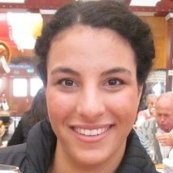
\includegraphics[width=\trainerIconWidth]{Champ.jpg} &
    \textbf{Ms. Katherine Champ}\newline
    Workshop Coordinator\newline
    Project Officer, Bioplatform Autralia Ltd.\newline
    \mailto{kchamp@bioplatforms.com}\\


  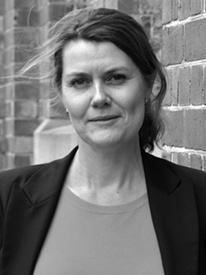
\includegraphics[width=\trainerIconWidth]{photos/VDam.jpg} &
    \textbf{Dr. Ellen Van Dam}\newline
    Workshop Coordinator\newline
    National Operation Manager, Bioplatform Autralia Ltd.\newline
    \mailto{evandam@bioplatforms.com}\\  
  
\end{longtable}
\end{center}



%
% Workshop Preamble
%
\input{015_preamble/preamble.tex}

%
% Start of modules
% Switch chapter styling to module
%
\chapterstyle{module}


%
% End of modules
% Switch back to normal workshop chapter styling
%
\chapterstyle{workshop}

\chapter{Space for Personal Notes or Feedback}
\clearpage

%
% Some empty ruled comments pages
%
\myruledpage{0cm}{1cm}
\myruledpage{0cm}{1cm}
\myruledpage{0cm}{1cm}
\myruledpage{0cm}{1cm}

\end{document}
